\section*{Om øvingen og innleveringen}

\begin{boxedminipage}{\textwidth}
    \begin{itemize}
      \setlength\itemsep{0mm}
    \item For å bli kjent med Simulink på en effektiv måte,
      er alle oppgavene i denne øvingen svært nyttige, og de vil
      fungere som et oppslagsverk for deg.

  \item For å tilrettelegge for at du skal gjøre flest mulig oppgaver,
    så skal du laste ned og pakke opp \fbox{\tt
      oving2\_skallfiler.zip} som inneholder:
    \begin{itemize}
    \item     Simulink-skallfilen
    \fbox{\tt oving2.slx} hvor deloppgavene a)-p)
    implementeres i egne subsystem
    \item den ferdige modellen \fbox{\tt  oving2\_oppg\_q.slx} for
      deloppgave q)  
  \item skallfilen   \fbox{\tt oving2\_data.m} som
  du må kjøre for 2i),  2o), 2p) og 2q).    
\end{itemize}
    Simulink-skallfilene er spesifisert med trapesmetoden  {\sf ode2 (Heun)} som
    integrasjons\-metode og tidsskritt $T_{s}$ lik 0.01 sekund.

\item  Resultater i scope kan du overføre til en MATLAB-figur med menyvalget
  \dbox{\tt File -->  Print to Figure}, som du igjen kan
     bruke \fbox{\tt LagreMinFigur} på, se prosedyre-boksen nedenfor.
      

    \item   {\color{red}  For å få øvingen godkjent må du gjøre følgende oppgaver:\\
      \fbox{a), c), d),  f), g), i), o), p), q) }}

        \item   Oppgavene 
          \fbox{b), e), h), j), k), l), m), n) } er også lærerike og nyttige, men frivillige.
Dette er markert i toppteksten.       

  \item   {\color{red}  For å ta eksamen i emnet  ELE130 så må denne øving være
  godkjent. Husk at øvingene må leveres individuelt.}


  \item Basis for denne øvingen er
    {\color{blue} kapittel 4  og 5} i  kompendiet. 

    \item På samme måte som i øving 1 finner du en {\LaTeX}-mal i filen 
    \fbox{\tt oving2\_Overleaf.zip}.

  \end{itemize}
  \end{boxedminipage}

 Så langt
det er mulig skal du benytte blokker fra {\sf Eget bibliotek}
  slik at nyttig informasjon om blokkene vises i blokkdiagrammet. Du skal 
  benytte {\sf Scope}-blokkene som heter {\sf Scope, tynne linjer}
  eller {\sf Scope, tykke linjer}  fra {\sf Eget bibliotek} til å
  vise resultatene i.
  Øvingen og skallfilen er organisert  i følgende deler/subsystem:
  \vspace*{-5mm}
  \begin{itemize}
%    \setlength\itemsep{0mm}
  \item ``Om {\sf Integrator}-blokken'', oppgave 2a) - 2e) 
  \item ``Om {\sf Sine Wave}-blokken'', oppgave 2f) - 2h) 
  \item ``Om {\sf Lookup Table}-blokken'',  oppgave 2i) - 2l) 
  \item ``Litt diverse'', oppgave 2m) - 2p)  
  \item ``PID-regulatoren'', oppgave 2q)  
  \end{itemize}


  
I mange av oppgavene skal du inkludere simuleringsresultatet i
innleveringen din og samtidig lese av verdier i MATLAB-figuren.
Prosedyren for å gjøre dette er som følger:
\begin{tcolorbox}[colback=yellow!5!white,colframe=yellow!75!black,
    title=Prosedyre for å lage figur fra
    Simulink-scope og deretter lese av verdier]
       \begin{itemize}
       \item Velg  \dbox{\tt File -->  Print to Figure} fra scopet. Vær
         klar over at eventuelle  avlesningene ved bruk av  {\sf Cursor
           Measurements} ikke blir med i MATLAB-figuren.
       \item Det å avlese/markere i MATLAB-figurer som er laget med utgangspunkt i et
         Simulinkscope gjøres ikke på samme måte som i vanlige
         MATLAB-figurer. Du må nemlig du bruke {\sf Data Cursor}-verktøyet vist i rød ring figuren
         under. For  å avlese mer enn ett punkt, husk å holde inne \dbox{\tt Shift}-knappen.
         \begin{figure}[H]
           \centering
           \scalebox{0.6}{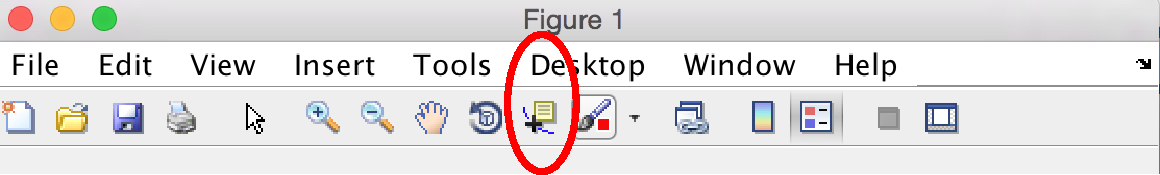
\includegraphics{data_cursor.pdf}}
           \caption{Trykk på knappen i rød ring for å lese av verdier på grafen i en
             figur som er eksportert fra Simulink.  }
         \end{figure}  

       \item Benytt deretter \fbox{\tt LagreMinFigur}-funksjonen til å lage en .pdf av
         figuren. 
       \end{itemize}
       
     \end{tcolorbox}

\label{page:prosedyre}

\newpage